\section{Routing Protocol for Low-Power and Lossy Networks (RPL)}

RPL is an distance-oriented vector routing protocol that builds a
Destination-Oriented Directed Acyclic Graph (DODAG) over IEEE
802.15.4 PHY/MAC layers and 6LoWPAN (IPv6 over Low-Power
Wireless Personal Area Networks) \cite{alexanderRPLIPv6Routing2012}.
It is primarily designed for Wireless
Sensor Networks (WSNs),
where multipoint-to-point traffic toward one or more roots is the
predominant communication pattern.
Routes in RPL are optimised for traffic to or from one or more
roots in the topology, while maintaining reliable and energy
efficient data collection. To maintain reliable and energy-efficient
data collection, RPL is designed to adapt to changing
network conditions, allowing nodes to switch routes when route
degradation is detected.

\subsection{Destination-Oriented Directed Acyclic Graph (DODAG)}
RPL organises nodes under a DODAG, with the WSN's sink
node often serving as the root of DODAG. In a multi-sink deployment,
each sink node serves as the root of its own separate DODAG.
Within a DODAG, each node maintains a rank value, which is an estimation of the
distance between itself and the DODAG
root, and forms a directed edge toward a parent with a lower rank,
creating a herarchy network toward the root, as illustrated in
Figure~\ref{fig:dodag-example}. Thus within this
hierachy, the root always has the lowest rank.

% TODO: include how DODAG maintain loop free

A node's rank is computed by an objective function (OF), which
translates one or more metrics into rank, and the RPL
specification does not mandate a single OF for all applications.
Instead, RPL separates its core routing procedures --- packet
forwarding and DODAG maintenance --- from route optimisation, leaving
the choice of OF open to fit the diverse requirements of LLNs, such as
minimising energy consumption, reducing latency, or improving link
quality. This separation is what gives RPL the flexibility to support
such a wide range of applications, since a DODAG can be optimised for
whichever metric best suits its deployment.

\begin{fig}[H]
    \begin{center}
        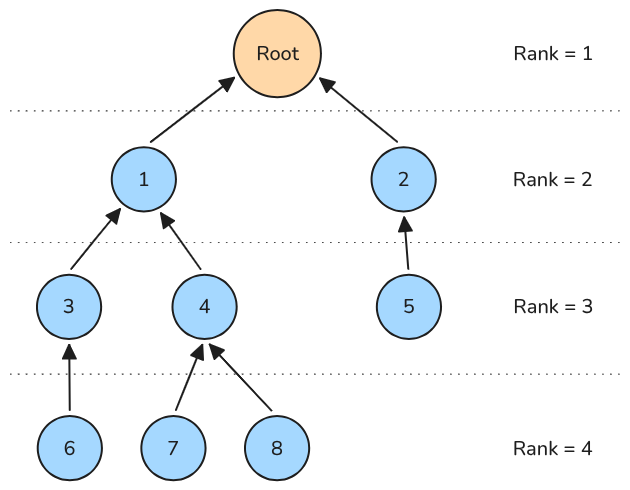
\includegraphics[width=0.6\textwidth]{assets/dodag.png}
        \caption{Example of a DODAG topology, showing nodes organised
        into a hierarchy rooted at the sink node.}
        \label{fig:dodag-example}
    \end{center}
\end{fig}

During DODAG construction, each node selects a parent from a pool of
candidate parents: neighbouring nodes that have already joined the
DODAG. The OF computes a candidate's resulting rank as
\[
    Rank(N) = Rank(P) + Rank\_Increase
\]
where $Rank(N)$ is the resulting rank of the node under consideration,
$Rank(P)$ is the rank already advertised by the candidate parent $P$,
and $Rank\_Increase$ is a positive value determined by the OF,
representing the cost of using $P$ as a parent. Because
$Rank\_Increase$ is always positive, a node's rank strictly increases
with each hop away from the root. The specific method used to compute
$Rank\_Increase$ and how parent is selected depends on the OF in use,
as discussed later in this chapter.

% There are four identifiers to define and maintain a topology in RPL shown in
% Table~\ref{tab:rpl-identifiers}.
% with RPLInstanceID and DODAGID used
% to identify a single DODAG in the network.
% % TODO: talk a bit more about why we have that many identifiers
%
% % TODO: talk about local and global repair
%
% % TODO: how to include identifier smoothly
% \begin{table}[h]
%     \caption{RPL DODAG identifiers} \label{tab:rpl-identifiers}
%     \begin{center}
%         \begin{tabular}{@{}p{0.25\linewidth}p{0.65\linewidth}@{}}
%             \hline
%             \textbf{Identifier} & \textbf{Description} \\
%             \hline
%             RPLInstanceID & The identifier of an RPL Instance, which may
%             span multiple DODAGs optimised for different applications. \\
%             DODAGID & The identifier of a specific DODAG within an RPL
%             Instance. \\
%             DODAG\-Version\-Number & The version number of a DODAG,
%             incremented by the root each time the DODAG is rebuilt to
%             distinguish between versions. \\
%             Rank & The estimated distance of a node from the DODAG
%             root; a node closer to the root has a lower rank. \\
%             \hline
%         \end{tabular}
%     \end{center}
% \end{table}

RPL introduces five types of control messages to form
and control DODAG, as specified in ICMPv6 via RFC 6550
\cite{alexanderRPLIPv6Routing2012}
\begin{itemize}
        % TODO: paraphrase this
    \item DODAG Information Object (DIO): carries information that
        allow nodes to discover a RPL instance, select parents and
        maintain the DODAG.
    \item DODAG Information Solicitation (DIS): a request message
        when a node want to join a DODAG
    \item Destination Advertisement Object (DAO): the node advertise
        itself to the root node, indicating that it has join DODAG
        and is reachable
    \item Destination Advertisement Object Acknowledgement (DAO-ACK):
        the acknowledgement of the root, confirming the downward path
        to the node
    \item CC: % TODO: what is this
\end{itemize}

To begin the DODAG forming process, the root node sends its DIO to
its neighbouring nodes, carrying RPL indentifiers and any
additional metrics required by the OF. Upon receiving DIO, a node
compares its rank with the advertised rank and filters out ranks that
are higher then its own to prevent loop formation, and then decides
whether to join the advertised DODAG or not.
In certain implementations, a node waits for several DIOs, building
the pool of candidate parents before deciding.
Afterward, the node computes the path cost of the
corresponding link for each candidate and determines the preferred
parent according the OF's policy.
Once a parent has been selected, the node broadcasts its own DIO to
advertise itself to its neighbours. This process is repated
outward through the network until every node has join the DODAG.
% TODO: may include diagram of how DIO transmission work

DIO is crucial in forming and maintaining DODAG, and DODAG requires
periodic DIOs to repair and update the conditions of the DODAG.
However, frequent DIO would be redudant in consistent network
conditions, thus RPL employs Trickle timer to regulate the emission of DIO.

% TODO: talk more about DAO
A node would send DAO message back to its parent or the root node to
establish downward communication.
In the DAO-ACK mode, a node wait
for the root node to send back DAO-ACK
before confirming that it is reachable and advertise DIO to surrounding nodes

% TODO: talk more about DIS
In addition for a node waiting to receive DIO to join DODAG, the node
can send DIS message to request DODAG information. When surrounding
nodes receive a DIS, it must unicast its DIO to that node, without
effecting the Trickle Timer policy. After receiving the unicasted
DIO, the node process the DIO as if it has receive a periodic DIO.

% TODO: write more about trickle timer
\subsection{Trickle Timer}
Trickle Timer is a scheduling algorithm based on consistency model.
The algorithm is structured in a way that would promptly send out DIO
during the formation process and would slow down when the DODAG has
been stablised.

adjusting the scheduling
regulates DIO transmission by adjusting the sending interval dynamically
based on the packets and network condition, ensuring timely DIO update
while reducing redundant message transmission \cite{rfc6206}.
The Trickle timer does this by evaluating the consistency of the
network message with its own state. However, the definition of
inconsistencies is left
for interpretation of the implementation. % TODO: give example of
% inconsistencies in RPL
In RPL specification, inconsistencies are defined as:
These inconsistencies$I$ include join new DODAG
version (e.g. new DODAGVersionNumber, new RPL instance, switching
parent), when % TODO: does switching parent reset DIO
nodes detect loop and additional inconsistencies according to the
implementation.
However, the specification leaves the implementation adds more
inconsistencies type when needed

When the network information is consistent, it
exponentially increases the transmission interval of DIO. However,
upon detecting inconsistencies, trickle timer reset its send interval
to boost DIO transmission to spread the latest information to the
rest of the DODAG.

Trickle Timer employs three configuration
parameters to determine the sending window of DIO: $I_{min}$, $I_{max}$ and $k$.
The maximum sending interval time is:
\[
    I_{max\_time} = I_{min} \times 2^{I_{max}}
\]

% TODO: give an example

Trickle timer set the initial sending interval $I$ in the range of
$[I_{min}, I_{max\_time}]$, usually the initial interval is set to $I = I_{min}$
% TODO: read more about trickle timer
The trickle timer will select a random time $t$ between $[I/2, I)$ as the
sending interval. When Trickle detects a consistent message, it will
increase the counter $c$,
At the time $t$, if the value of $c$ is less than the
redundancy constant $k$, the trickle transmits the message, otherwise
it would suppress the transmission.
After the interval $I$, Trickles double the time of the interval up
to $I_{max\_time}$ i.e. $I = max(I \times 2, I_{max\_time})$

Upon detecting inconsistent messages, The interval $I$ is reset to
$I_{min}$ to increase the DIO sending rate.

\begin{table}
    \caption{Trickle Timer Parameters}\label{tab:tricker_timer_params}
    \begin{center}
        \begin{tabular}[c]{@{}p{0.22\linewidth}p{0.10\linewidth}p{0.58\linewidth}@{}}
            \hline
            \textbf{Parameter} & \textbf{Symbol} & \textbf{Description} \\
            \hline
            Min interval length & $I_{min}$ & The minimum sending
            interval between two messages \\ % TODO: problably fix this
            Max interval length & $I_{max}$  & The maximum number of
            times that the sending interval can double \\
            DIO redundancy constant & $k$ & The number of consistent
            DIOs before suppresses its own DIO transmission \\
            \hline
        \end{tabular}
    \end{center}
\end{table}

\subsection{Communication Patterns}
% TODO: probably combine this with DIO transmission and DAO transmission
There are two types of communication patterns in RPL: upward route
and downward route
\subsubsection{Upward Route}
A node forwards packets toward the sink by relaying them to its
parent, which in turn relays them further up the tree until they reach the root.
Since a parent's rank is always lower than its child's and the root
rank is lowest, this process cannot get stuck in an endless cycle.

\subsubsection{Downward Route}
The downward are supported to P2MP and P2P route, in which the
destination is not the root node. In this pattern, the node sends DAO
to its preferred parent in a unicast manner

% TODO: study the storing mode more
In this pattern, the RPL specification defines two mode: storing mode
and non-storing mode. In storing mode, the downward routing tables
are included in each nodes
However, in non-storing mode, the downward routing tables are stored
only in the DODAG root. This means that P2P communication need to be
forwarded to the root node, where the root would then formulate the
routing path to the downward node.

% TODO: clarify this
The specification also opens option to specify DAO-ACK or not. A node
would only consider reachable only after it has received the DAO-ACK.

\subsection{OF0 and MRHOF}

Up to now, the IETF ROLL working group has standardised only two
objective functions: Objective Function Zero (OF0) \cite{rfc6552} and
Minimum Rank with Hysteresis Objective Function (MRHOF) \cite{rfc6719}.

% TODO: talk more about step of rank
OF0 was developed to be a simple objective function that utilise step
of rank, which is an intermediate computation based on link
properties of a certain neighbour.
, computing
$Rank\_increase$ as follow
\[
    Rank\_Increase = ( Rf \times Sp + Sr) \times Min\_Rank\_Increase
\]
where $Rf$ (Rank Factor) is a small positive integer used to scale
the step of rank; $Sp$ (Step of Rank) is an integer value
representing hop count in
abstract sense; and $Sr$ (Stretch of Rank) is used to inflate
$Rank\_Increase$ for
hysteresis preventing the OF from switching parents constantly.
We can select
OF0 parameters by
selecting $Rf = 1$, $Sp = 1$ and $Sr = 0$, which reduces
$Rank\_Increase$ to a simple fixed per-hop increment of 256. However,
The specification of OF0 strongly recommend computing step of rank
from Expected Transmission Count (ETX) to avoid blind hop count
measure, where it would select furthest
node to reduce the number of hops, leading to noisy and lossy link

OF0 can be regarded as implicitly using hop count as
routing metric. This mean that the traffic from OF0 follow the shortest path
to root without considering any load balancing requirement.
However, this also means that OF0 does not consider other link
qualities such as latency, energy residual in its calculation as well
as might choose worse off route but have the shortest hop count to root.
This led to the introduction a more sophisticated MRHOF.

In contrast, MRHOF propose multiple thresholds call hysteresis for
path cost and time
. In path cost threshold, unless the
potential node is better than the current parent by a threshold, it
will stick with the current parent. However, after the time
threshold, if that node is still better then the node will switch
parent. This would allows a more stabilised DODAG. Additionally,
MHROF allow choosing one from various metrics as the determing factor.

The default metric of MRHOF is Expected Transmission Count (ETX)
metric. The main goal of ETX is to select routes with high end-to-end
through put:
\[
    ETX = \frac{1}{D_t \times D_a}
\]
where $D_t$ is the probability that the receiving node receives the
packet and $D_a$ is the probability that the transmitting node
receives acknowledgement packet is successful. So ETX is the average
number of packets need to send and acknowledgement.
Since ETX is a floating point number while devices RPL operates on do
not generally support floating point arithmeic. The specifcation
indicates that 128 would be 1.0 ETX, improving the performace with
bitshift instead of expensive division.

% TODO: what word to describe route need less packets TX
In essense, using ETX as metrics focus on more transmission-efficient route.

There are two thresholds in MRHOF, rank threshold and time threshold.
The specification define $PARENT\_SWITCH\_THRESHOLD$ as the minimum
path cost improvement before deciding to switch.
There is time threshold, meaning that if a node consistently perform
better but not more than the ETX threshold, it still switch.

% TODO: include other metric container
The specification also open the choices of the routing metrics to energy,...
However, ETX is the more popular choice when it comes to MHROF.

Thanks to the flexibility of DIO header option.
% TODO: talk about the flexiblity of DIO

\section{Load Balancing in RPL}
Load balancing is an important issue in WSNs since devices are
expected to operate on battery for a long period of time. Some nodes
are used more frequently than others, especially the nodes near the
root, and exhaust their energy rapidly. These also includes when
there is an imbalance the traffic rate between node, where certain
nodes have higher data traffic than others e.g. videos or images,
thus selecting one parent would exhaust the possible routes to the parent node.

In this sense, load balancing is about distributing load from the
leaf to root node so that the node within the same hop share the
loads more evenly

These have to account for bursty traffic

% TODO: define what is load balancing
Despite that, RPL does not consider load balancing since it is
oriented to handling
low data traffic. Therefore, the network suffers in terms of latency,
delivery ratio and energy consumption under imbalance load senerios.

This is where OF0 and MRHOF fall short as they only consider one
metric: hop count and ETX. This does not capture the different
load of each node. Generally, ETX value does not change much when a
node experience heavy load \cite{kimQURPLQueueUtilization2015}

Another problem in load balancing is Thundering Herd problem, when a new node join the DODAG and advertise its existence. Since this node does not have any load, the neighbouring nodes would then choose this as their prefered parents, potentially overloading this node. While leaving their current parent free of load. When the current parent advertise itself, all the node would then switch, thus creating switch back and forth.
% TODO: insert image for thundering herd

% TODO: include other problems in load balancing as well

